\documentclass[12pt,a4paper]{article}

\usepackage[margin=1in]{geometry}
\usepackage[T1]{fontenc}
\usepackage[utf8]{inputenc}
\usepackage{lmodern}
\usepackage{textcomp}
\usepackage{parskip}
\usepackage{graphicx}
\usepackage{setspace}
\usepackage{float}
\usepackage[section]{placeins}
\usepackage{booktabs}
\usepackage{array}
\usepackage{longtable}
\usepackage{caption}
\usepackage{subcaption}
\usepackage{pgfgantt}
\usepackage{enumitem}
\usepackage{amsmath,amssymb}
\usepackage{siunitx}
\usepackage[hidelinks]{hyperref}

\newcolumntype{L}[1]{>{\raggedright\arraybackslash}p{#1}}
\renewcommand{\arraystretch}{1.35}
\captionsetup{font=small,labelfont=bf,skip=6pt}
\setlist[itemize]{topsep=2pt,itemsep=2pt,parsep=0pt,leftmargin=1.5em}
\sisetup{detect-weight=true, detect-family=true}

% Gantt chart styles (Section~\ref{sec:gantt})
\definecolor{ganttpast}{HTML}{8FC98F}
\definecolor{ganttnow}{HTML}{F5A25D}
\definecolor{ganttnext}{HTML}{DADADA}
\ganttset{
	gantt style/.style={
		time slot format=isodate, x unit=0.045cm, y unit title=0.45cm,
		y unit chart=0.335cm, hgrid={*1{black!8}}, vgrid={*6{draw=none}, *1{black!12}},
		title/.append style={draw=black!40, fill=black!6},
		title label font=\scriptsize, bar label font=\scriptsize,
		milestone label font=\scriptsize, group label font=\scriptsize\bfseries,
		bar height=0.55, bar/.append style={draw=black!50},
		group/.append style={fill=black!65, draw=none}, group height=0.25,
		group right shift=0, group left shift=0, group top shift=0.4,
		milestone left shift=-2, milestone right shift=2,
		milestone/.append style={draw=black!60},
		vrule/.append style={draw=red!70!black, dashed, thick},
		vrule label font=\scriptsize\bfseries\color{red!70!black},
	},
	gpast/.style={bar/.append style={fill=ganttpast}, milestone/.append style={fill=ganttpast}},
	gnow/.style={bar/.append style={fill=ganttnow}, milestone/.append style={fill=ganttnow},
		bar label font=\scriptsize\bfseries, milestone label font=\scriptsize\bfseries},
	gnext/.style={bar/.append style={fill=ganttnext}, milestone/.append style={fill=ganttnext}},
}
\DeclareRobustCommand{\ganttkey}[1]{\tikz[baseline=-0.6ex]\fill[#1, draw=black!50] (0,-0.12) rectangle (0.35,0.12);}

\begin{document}

%---------------------------------------------------------------- title page --
% Cover from Proposal.tex (ISE format), retitled for the progress report.
\begin{titlepage}
\centering
\setstretch{1.0}
\vspace*{0cm}

{\Large\bfseries Capstone Design Project I\par}
\vspace{0.3cm}
{\large Progress Report\par}

\vspace{0.6cm}

\includegraphics[width=3.2cm]{image/chula_eng_logo.png}\par
\vspace{0.6cm}

{\Large\bfseries A Modular Self-Reconfigurable Robot (MSRR)\\[0.35em]
for Search and Space Exploration\par}

\vspace{0.7cm}
{Submitted to the\par}
{Project Committee appointed by the\par}
{International School of Engineering (ISE)\par}
{Faculty of Engineering, Chulalongkorn University\par}

\vspace{0.6cm}
{\bfseries Project Advisors\par}
\vspace{0.35cm}
{Asst.\ Prof.\ Paulo Fernando Rocha Garcia, Ph.D.\par}
{Asst.\ Prof.\ Surat Kwanmuang, Ph.D.\par}

\vspace{0.6cm}
{\bfseries Submitted By\par}
\vspace{0.45cm}
\begin{tabular}{@{}l@{\hspace{2em}}l@{}}
Kittivut Pipattanachaiyapong  & 6638019121 \\
Krin Kaweewongsonthorn        & 6638027121 \\
Pakapol Kijsupanont           & 6638172421 \\
Phattharamon Sukvivatn        & 6638178221 \\
\end{tabular}

\vfill
{\footnotesize 1/2026: 2147498 Capstone Design Project I\par}
{\footnotesize Robotics and Artificial Intelligence Engineering (International
Program)\par}
{\footnotesize International School of Engineering (ISE), Faculty of Engineering,\par}
{\footnotesize Chulalongkorn University\par}
\end{titlepage}

% ================================================================
\section{Project Timeline}
% ================================================================

\begin{itemize}
	\item \textbf{Completed:} Project concept, objectives, literature review, and
	      phased system architecture established.
	\item \textbf{In progress:} Phase A --- single-module locomotion, sensing,
	      communication, and simulation baseline.
	\item \textbf{Next:} Phase B --- EP-Face docking, task-oriented
	      reconfiguration, and simple assembled locomotion.
\end{itemize}

% ================================================================
\section{Project Phases}
% ================================================================

\subsection{Phase A}
External perception and computation. Develop the mechanically homogeneous
module, differential-drive locomotion, joint control, odometry, and
module-to-commander communication. Validate the module and physics twin before
physical docking is introduced.

\subsection{Phase B}
Docking and task-oriented reconfiguration. Add the electropermanent EP-Face
connectors, infrared alignment, and connector-state feedback. Extend the
reconfiguration pipeline with task assignment, parallel assembly sequencing,
and selection from a library of feasible configurations.

\subsection{Phase C}
Onboard perception with external computation. Mount a monocular RGB camera and
an $8\times8$ multi-zone ToF sensor on the leader module. Estimate obstacle
geometry and traversability locally, while transmitting sensor data to an
external computer for processing.

\subsection{Phase D}
Fully onboard perception and computation. Move the perception and
configuration-selection pipeline onto a coordinator module using an embedded
compute board. Close the perceive--select--reconfigure--traverse loop on
hardware without external localisation or computation.

\clearpage
% ================================================================
\section{Gantt Chart}
\label{sec:gantt}
% ================================================================

Task schedule from the team Notion timeline (as of 25~Sep~2026), grouped by phase.

\begin{figure}[H]
\centering\scriptsize
\begin{ganttchart}[gantt style]{2026-08-17}{2027-01-17}
\gantttitlecalendar{year, month=shortname} \\
\ganttgroup{Phase A --- Locomotion, sensing and communication}{2026-08-28}{2027-01-09} \\
\ganttbar[gnow]{(Phase\_A\_1) Planning/ Trade Study}{2026-08-28}{2026-09-30} \\
\ganttmilestone[gpast]{MILESTONE - Proposal submission}{2026-08-28} \\
\ganttbar[gpast]{Module design Mechanic Draft 1 (CAD)}{2026-08-28}{2026-09-17} \\
\ganttbar[gnow]{Module design Mechanic Draft 1 (FAB) Draft\_1}{2026-09-18}{2026-10-12} \\
\ganttbar[gnow]{(sim) export URDF to gazebo, controller and locomotion}{2026-09-25}{2026-10-08} \\
\ganttmilestone[gnow]{MILESTONE - First progress report}{2026-09-25} \\
\ganttbar[gnext]{(Phase\_A\_1) Part Ordering/Shipping}{2026-10-01}{2026-10-15} \\
\ganttbar[gnext]{Control board and firmware}{2026-10-01}{2026-10-10} \\
\ganttbar[gnext]{Power, Main Board PCB Designing}{2026-10-01}{2026-10-15} \\
\ganttbar[gnext]{Gear and Shaft Print Testing and Redesign}{2026-10-05}{2026-10-25} \\
\ganttbar[gnext]{(sim) Implement Reconfiguration planning}{2026-10-09}{2026-11-03} \\
\ganttbar[gnext]{(sim) Navigation and avoidance with known coordinate}{2026-10-09}{2026-10-21} \\
\ganttbar[gnext]{Basic Locomotion Testing}{2026-10-13}{2026-10-20} \\
\ganttbar[gnext]{(Phase\_A\_1) Testing}{2026-10-16}{2026-10-20} \\
\ganttbar[gnext]{Power, Main Board PCB FAB + Part Ordering}{2026-10-16}{2026-10-29} \\
\ganttbar[gnext]{(real) Localization and navigation from camera}{2026-10-23}{2026-11-03} \\
\ganttmilestone[gnext]{MILESTONE - Second progress report}{2026-10-23} \\
\ganttbar[gnext]{Power, Main Board Testing}{2026-10-30}{2026-11-12} \\
\ganttbar[gnext]{Radio link and protocol}{2026-10-30}{2026-11-12} \\
\ganttbar[gnext]{UWB \& Radio link wifi testing (Dev board)}{2026-10-30}{2026-11-12} \\
\ganttbar[gnext]{low level control + Sensing IMU Encoder (Dev board)}{2026-10-30}{2026-11-12} \\
\ganttbar[gnext]{(real) Implement Reconfiguration planning}{2026-11-04}{2026-11-18} \\
\ganttbar[gnext]{Connector FAB (EP-Face) (1)}{2026-11-15}{2026-11-30} \\
\ganttbar[gnext]{Connector design (EP-Face)}{2026-12-11}{2027-01-09} \\
\ganttgroup{Phase B --- Docking and task-oriented reconfiguration}{2026-09-22}{2027-01-03} \\
\ganttbar[gnow]{EP Research and Face Design}{2026-09-22}{2026-09-30} \\
\ganttbar[gnext]{EP Face Part Ordering}{2026-10-01}{2026-10-14} \\
\ganttbar[gnext]{IR Face Design}{2026-10-01}{2026-10-09} \\
\ganttbar[gnext]{IR Face Part Ordering}{2026-10-10}{2026-10-23} \\
\ganttbar[gnext]{EP Face 1st Test}{2026-10-15}{2026-10-28} \\
\ganttbar[gnext]{IR 1st test}{2026-10-24}{2026-11-06} \\
\ganttbar[gnext]{In-Wheel (EP and IR) Board Designing}{2026-10-29}{2026-11-11} \\
\ganttbar[gnext]{(sim) urdf add contact face}{2026-11-05}{2026-11-18} \\
\ganttbar[gnext]{Contract face testing}{2026-11-13}{2026-11-26} \\
\ganttbar[gnext]{In-Wheel (EP and IR) Board FAB + Part Ordering}{2026-11-13}{2026-11-26} \\
\ganttmilestone[gnext]{MILESTONE - Draft final report}{2026-11-18} \\
\ganttbar[gnext]{(sim) precision docking with self alignment}{2026-11-20}{2026-12-03} \\
\ganttbar[gnext]{MILESTONE - Final presentation}{2026-11-22}{2026-12-03} \\
\ganttbar[gnext]{In-Wheel (EP and IR) Board Testing}{2026-11-27}{2026-12-10} \\
\ganttbar[gnext]{Locomotion with contact face testing}{2026-11-27}{2026-12-10} \\
\ganttbar[gnext]{(real) Reconfiguration planning with precision docking}{2026-12-04}{2026-12-17} \\
\ganttmilestone[gnext]{MILESTONE - Final report (Project I)}{2026-12-10} \\
\ganttbar[gnext]{W5 Assembled gaits, PPO training}{2026-12-11}{2027-01-03} \\
\ganttbar[gnext]{W6 IR alignment and docking}{2026-12-11}{2026-12-27} \\
\ganttbar[gnext]{W7 EP-Face build and characterisation}{2026-12-11}{2027-01-03} \\
\ganttbar[gnext]{W8 Configuration library}{2026-12-11}{2026-12-27}
\ganttvrule{Today (25 Sep)}{2026-09-25}
\end{ganttchart}
\caption{Project I schedule (Phases A--B). \ganttkey{ganttpast}~Completed \quad \ganttkey{ganttnow}~In progress \quad \ganttkey{ganttnext}~Upcoming; dashed line marks the report date.}
\label{fig:gantt-ab}
\end{figure}

\begin{figure}[H]
\centering\scriptsize
\begin{ganttchart}[gantt style]{2026-12-07}{2027-04-30}
\gantttitlecalendar{year, month=shortname} \\
\ganttgroup{Phase C --- Onboard perception, external computation}{2026-12-13}{2027-03-05} \\
\ganttbar[gnext]{(sim) Environment classification}{2026-12-13}{2027-01-18} \\
\ganttbar[gnext]{(sim) onboard perception obstacle avoidance and navigation}{2026-12-13}{2026-12-31} \\
\ganttbar[gnext]{Onboard perception testing}{2026-12-24}{2027-01-06} \\
\ganttbar[gnext]{(Real) Onboard Perception nav and configuration planning}{2027-01-01}{2027-01-18} \\
\ganttbar[gnext]{Inductive Encoder Designing}{2027-01-01}{2027-01-20} \\
\ganttbar[gnext]{Locomotion, Planning with internal Perception (IR and UWB)}{2027-01-03}{2027-01-31} \\
\ganttbar[gnext]{W9 Camera and ToF integration}{2027-01-04}{2027-02-12} \\
\ganttbar[gnext]{W5 Policy training on held-out params}{2027-01-11}{2027-02-26} \\
\ganttbar[gnext]{W8 Obstacle state to configuration}{2027-01-18}{2027-03-05} \\
\ganttbar[gnext]{(sim) Configuration lookup table}{2027-01-19}{2027-02-01} \\
\ganttbar[gnext]{Inductive Encoder FAB + Part Ordering}{2027-01-21}{2027-02-10} \\
\ganttbar[gnext]{W9 Terrain and traversability pipeline}{2027-01-25}{2027-03-05} \\
\ganttbar[gnext]{(Real) environment adaptation}{2027-02-02}{2027-02-28} \\
\ganttbar[gnext]{Inductive Encoder Testing}{2027-02-11}{2027-02-28} \\
\ganttbar[gnext]{MILESTONE - Phase C evaluation}{2027-03-01}{2027-03-05} \\
\ganttgroup{Phase D --- Fully onboard perception and computation}{2027-01-21}{2027-04-30} \\
\ganttbar[gnext]{PCB for CM5 Designing}{2027-01-21}{2027-02-04} \\
\ganttbar[gnext]{PCB for CM5 Designing FAB + Part Ordering}{2027-02-05}{2027-02-18} \\
\ganttbar[gnext]{W10 Compute module bring-up}{2027-02-15}{2027-03-19} \\
\ganttbar[gnext]{CM5 with RGBD and TOF Testing}{2027-02-19}{2027-03-04} \\
\ganttbar[gnext]{Onboard Odometry with no camera testing}{2027-02-22}{2027-03-11} \\
\ganttbar[gnext]{W4 Onboard odometry, drop VICON}{2027-02-22}{2027-04-02} \\
\ganttbar[gnext]{(sim) local interaction to reorganize (concept)}{2027-03-01}{2027-04-09} \\
\ganttbar[gnext]{Full testing internal computation}{2027-03-01}{2027-04-02} \\
\ganttbar[gnext]{Internal Computation}{2027-03-01}{2027-03-14} \\
\ganttbar[gnext]{W10 Quantised inference on module}{2027-03-08}{2027-04-09} \\
\ganttbar[gnext]{MILESTONE - Loop closed on hardware}{2027-04-05}{2027-04-09} \\
\ganttbar[gnext]{MILESTONE - Final evaluation (Project II)}{2027-04-26}{2027-04-30}
\end{ganttchart}
\caption{Project II schedule (Phases C--D). All tasks upcoming (\ganttkey{ganttnext}).}
\label{fig:gantt-cd}
\end{figure}

% ================================================================
\section{Module CAD Design}
\label{sec:module-cad-design}
% ================================================================

The design is based on SMORES-EP \cite{tosun2016} (originally \SI{80}{mm}), scaled to a $100 \times 100 \times 100$\,mm envelope for additional packaging space.

\begin{figure}[!htbp]
	\centering
	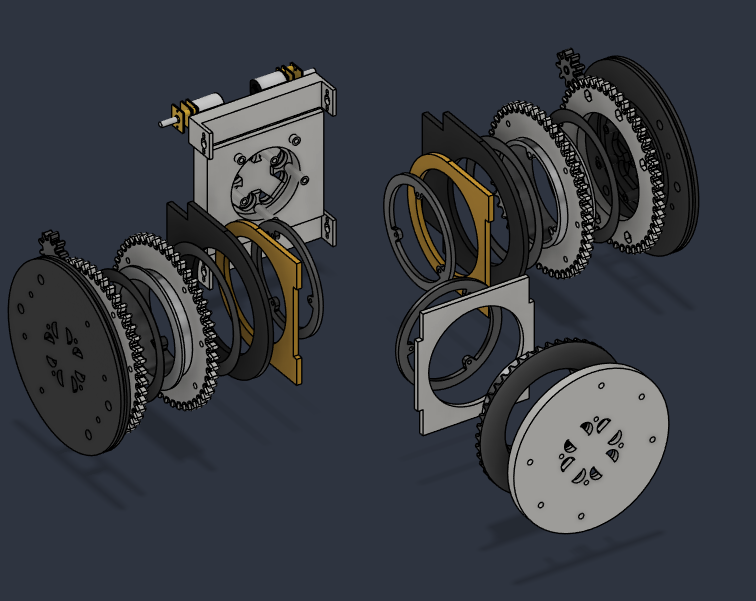
\includegraphics[width=0.6\textwidth]{image/exploded_view.png}
	\caption{Exploded view of the module.}
	\label{fig:exploded-view}
\end{figure}

\begin{figure}[!htbp]
	\centering
	\begin{subfigure}[b]{0.40\textwidth}
		\centering
		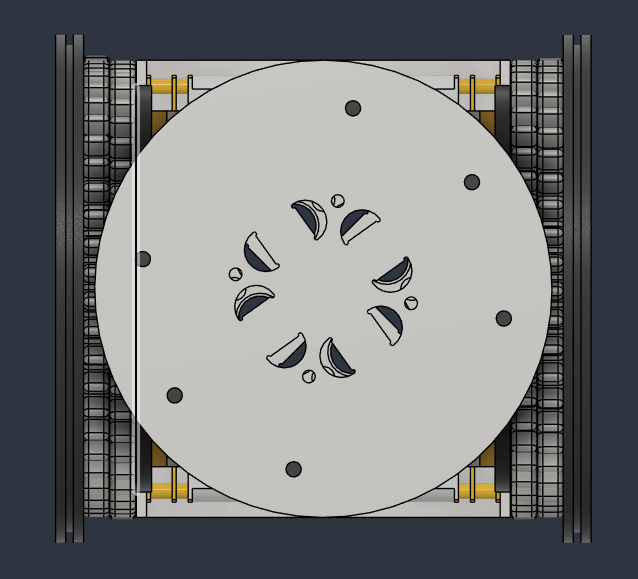
\includegraphics[width=\linewidth]{image/front.png}
		\caption{Front view.}
		\label{fig:cad-front}
	\end{subfigure}
	\hfill
	\begin{subfigure}[b]{0.40\textwidth}
		\centering
		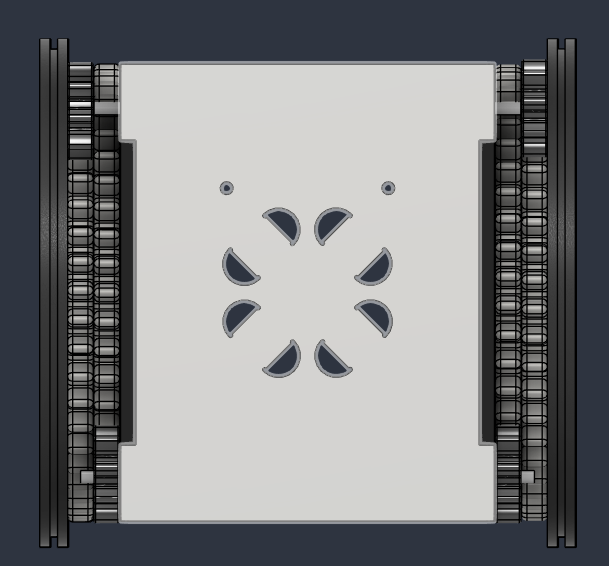
\includegraphics[width=\linewidth]{image/rear.png}
		\caption{Rear view.}
		\label{fig:cad-rear}
	\end{subfigure}
	\par\vspace{6pt}
	\begin{subfigure}[b]{0.40\textwidth}
		\centering
		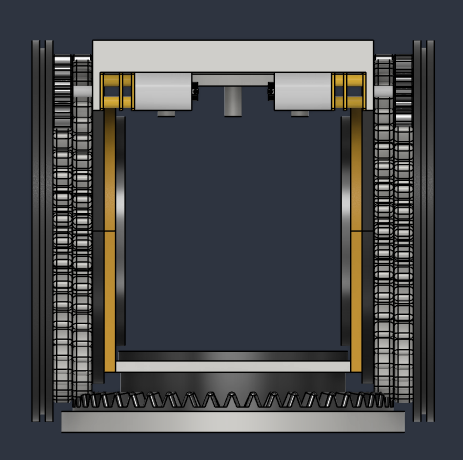
\includegraphics[width=\linewidth]{image/top.png}
		\caption{Top view.}
		\label{fig:cad-top}
	\end{subfigure}
	\hfill
	\begin{subfigure}[b]{0.40\textwidth}
		\centering
		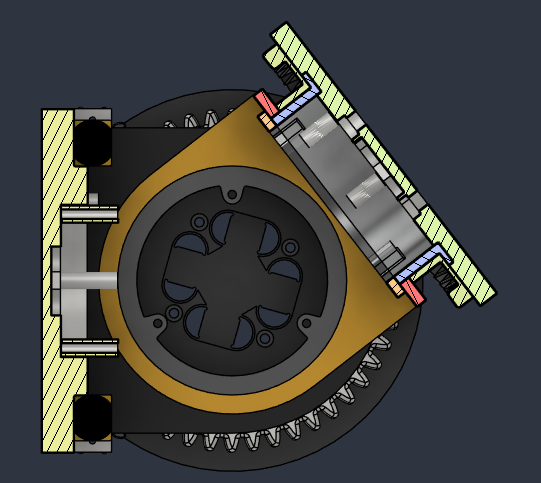
\includegraphics[width=\linewidth]{image/tilt.png}
		\caption{Tilted sectional view.}
		\label{fig:cad-tilt}
	\end{subfigure}
	\caption{Module CAD views.}
	\label{fig:cad-views}
\end{figure}

% ----------------------------------------------------------------
\subsection{Gear Train Design}
\label{sec:gear-design}

\begin{figure}[!htbp]
	\centering
	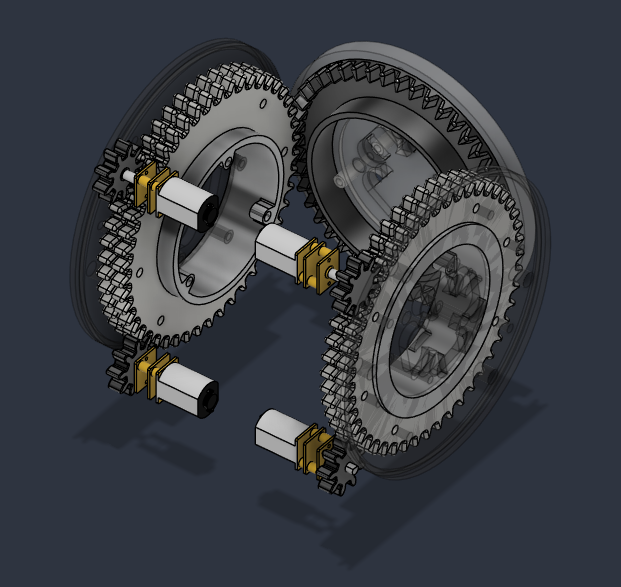
\includegraphics[width=0.6\textwidth]{image/GearCAD.png}
	\caption{CAD view of the gear train and motor arrangement.}
	\label{fig:cad-gear-train}
\end{figure}

% \begin{figure}[H]
% 	\centering
% 	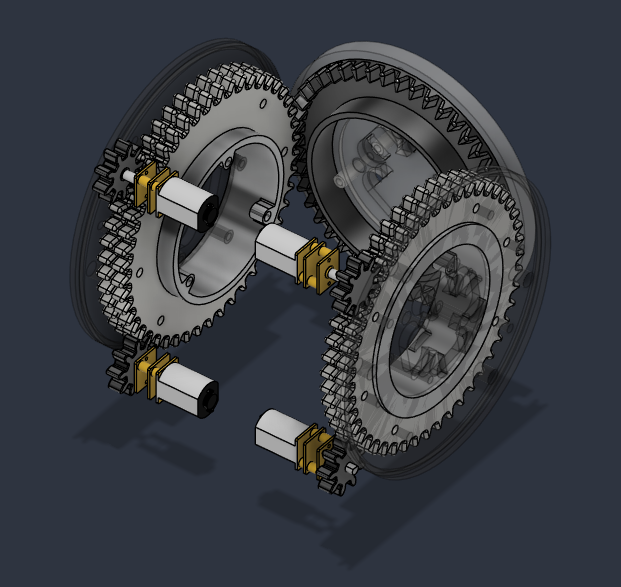
\includegraphics[width=0.6\textwidth]{image/GearCAD.png}
% 	\caption{Additional CAD view of the gear assembly.}
% 	\label{fig:cad-additional-view}
% \end{figure}

\subsubsection{SMORES-EP Reference Baseline}

The original SMORES-EP gear train was reverse-engineered from published data (Table~\ref{tab:smores-ref}), yielding module $m = 1.4$, pitch diameter \SI{67.2}{mm}, and stage ratio $48/9 = 5.33$.

\begin{table}[H]
	\centering
	\caption{Reconstructed SMORES-EP reference parameters.}
	\label{tab:smores-ref}
	\begin{tabular}{ll}
		\toprule
		\textbf{Parameter} & \textbf{SMORES-EP} \\
		\midrule
		Module envelope & $80 \times 80 \times 80$\,mm \\
		Spur gear       & 48 teeth \\
		Crown gear      & Same part as spur, used at \SI{90}{\degree} \\
		Pinion          & 9 teeth \\
		Gearbox         & 298:1 \\
		\bottomrule
	\end{tabular}
\end{table}

\subsubsection{New Gear Geometry}

The \SI{100}{mm} envelope allows a max spur gear OD of \SI{90}{mm}. The 5.33:1 ratio was preserved (64/12 teeth) to keep the gearbox selection, SMORES-EP benchmarks, and control firmware valid. The 64/12 pair was chosen over 48/9 because 12 teeth reduces undercutting, improves contact ratio, and provides a larger pinion bore.

Unlike SMORES-EP (which reuses a spur gear as a crown gear), this design uses a \textbf{true crown (face) gear} for better load distribution. The crown gear was sized to \SI{84}{mm} OD (46 teeth, $m = 1.75$) after a \SI{90}{mm} first attempt interfered with surrounding components.

This creates a \textbf{module mismatch} ($m = 1.36$ spur vs.\ $m = 1.75$ crown) --- an accepted compromise since both diameters and tooth counts are fixed by packaging and ratio constraints. The crown dedendum was reduced to \SI{2.15}{mm} (from standard \SI{2.19}{mm}) to clear tip interference.

\begin{table}[H]
	\centering
	\caption{Final gear train parameters.}
	\label{tab:final-params}
	\begin{tabular}{llllp{4.0cm}}
		\toprule
		\textbf{Component} & \textbf{Teeth} & \textbf{Module} & \textbf{OD} & \textbf{Notes} \\
		\midrule
		Wheel spur gear & 64 & \num{1.36} & \SI{90}{mm} &
		\SI{5}{mm} face width, bolt holes in web \\
		\addlinespace
		Pinion (both) & 12 & \num{1.36} & \SI{19.04}{mm} &
		Through-bore (pan/tilt) or blind (wheel) \\
		\addlinespace
		Crown gear & 46 & \num{1.75} & \SI{84}{mm} &
		Dedendum \SI{2.15}{mm}; true face-gear \\
		\bottomrule
	\end{tabular}
\end{table}

Common: \SI{20}{\degree} pressure angle, \SI{0.2}{mm} backlash, \SI{0.3}{mm} root fillet, \SI{0.1}{mm} bore tolerance. All gears generated via Fusion~360. Material: 3D-printed nylon.

\subsubsection{Drivetrain Architecture}

Four motors drive four spur gears:
\begin{itemize}
	\item \textbf{Outer two} --- each drives a wheel (differential-drive locomotion).
	\item \textbf{Inner two} --- both mesh with a single crown gear:
	      same direction $\rightarrow$ \textbf{pan};
	      opposite directions $\rightarrow$ \textbf{tilt}.
\end{itemize}

\subsubsection{Status}

All geometry is CAD-only. \textbf{No parts have been printed or tested.} Priority next steps: print first articles, verify spur/crown mesh despite module mismatch, check 12-tooth pinion undercut at print tolerances, and validate backlash and bore fit.

% ----------------------------------------------------------------
\subsection{Outer Wheels}

Two independently driven wheels (\SI{100}{mm} diameter) with NBR N70 O-ring tire groove (\SI{1.5}{mm} cross-section), EP-magnet docking space, and PCB mounting posts.

\begin{figure}[!htbp]
	\centering
	\begin{subfigure}[b]{0.45\textwidth}
		\centering
		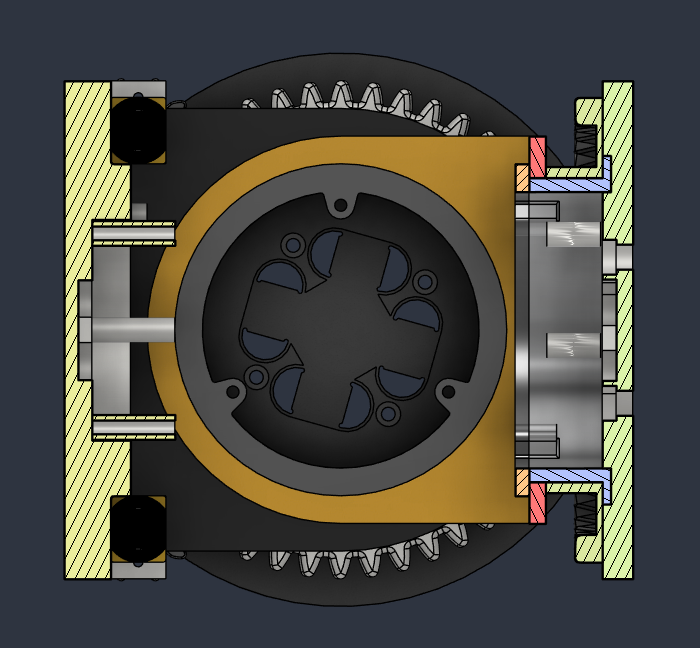
\includegraphics[width=\linewidth]{image/inside_wheel.png}
		\caption{Interior view (wheel and drivetrain).}
		\label{fig:cad-inside-wheel}
	\end{subfigure}
	\hfill
	\begin{subfigure}[b]{0.45\textwidth}
		\centering
		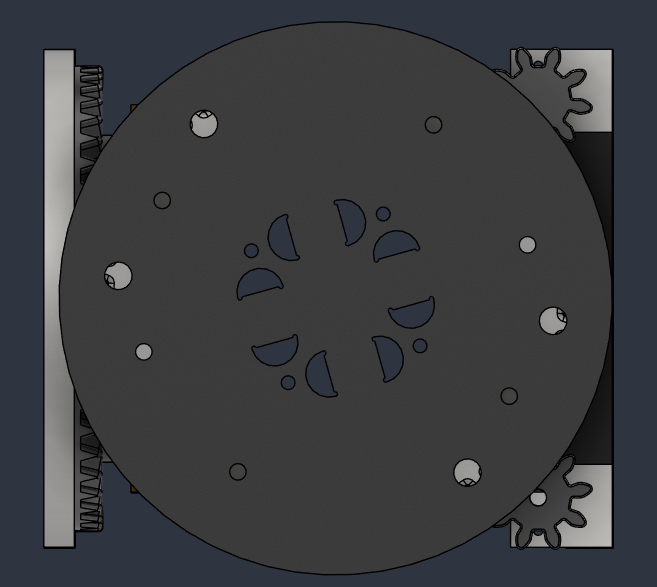
\includegraphics[width=\linewidth]{image/outside_wheel.png}
		\caption{Exterior view (wheel and module).}
		\label{fig:cad-outside-wheel}
	\end{subfigure}
	\caption{Outer wheel CAD.}
	\label{fig:cad-wheels}
\end{figure}

\subsection{Pan Face}

\SI{90}{mm} diameter, no O-ring groove. Includes EP-magnet docking space.

\subsection{Tilt Face}

Approximately $90 \times 71.6$\,mm rectangular part with EP-magnet docking space and an additional motor mount.

\clearpage
% ================================================================
\section{Electronics}
\label{sec:electronics}
% ================================================================

\subsection{Phased Electronics Plan}

Electronics are built incrementally across project phases:

\begin{itemize}
  \item \textbf{Phase A-1:} COTS parts --- 2S battery, 4-channel motor driver with MCU, ESP32-C3 for Wi-Fi.
  \item \textbf{Phase A:} Custom PCBs --- power board (buck, LDO, 4$\times$ H-bridge with current sensing) and main board (STM32G474, IMU, UWB, Wi-Fi).
  \item \textbf{Phase B:} In-wheel PCB with EP-Face circuitry and IR contact-alignment, connected via slip ring.
  \item \textbf{Phase C:} RGB-D/ToF camera (Sipeed MaixSense A075V) + wheel encoder added; compute still external.
  \item \textbf{Phase D:} Raspberry Pi CM5 on custom carrier PCB moves compute onboard.
\end{itemize}

\begin{figure}[!htbp]
  \centering
  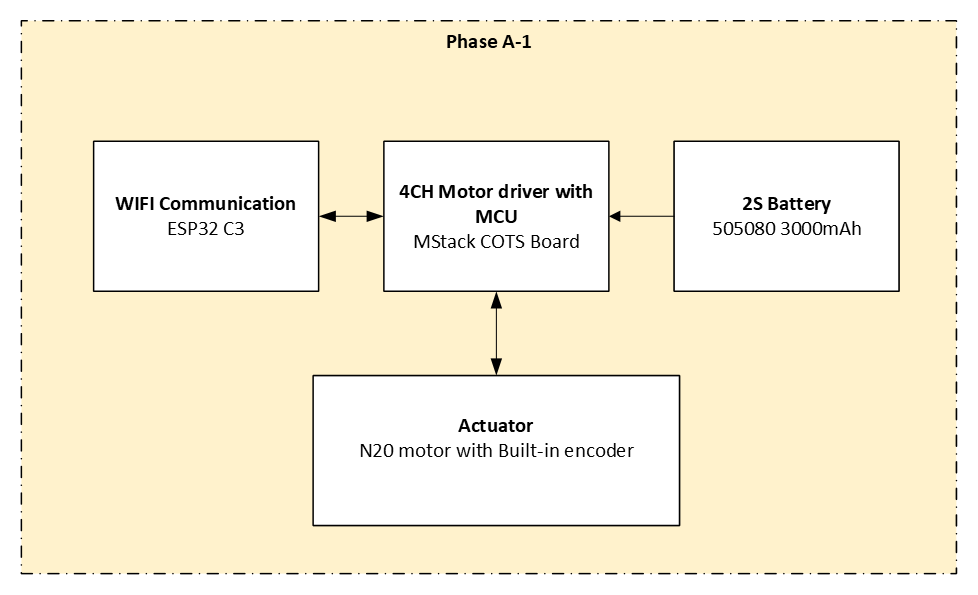
\includegraphics[width=0.78\textwidth]{image/Phase_A_1_Diagram.png}
  \caption{Phase A-1 electronics block diagram.}
  \label{fig:phase-a1}
\end{figure}

\begin{figure}[!htbp]
	\centering
	\begin{subfigure}[b]{\textwidth}
		\centering
		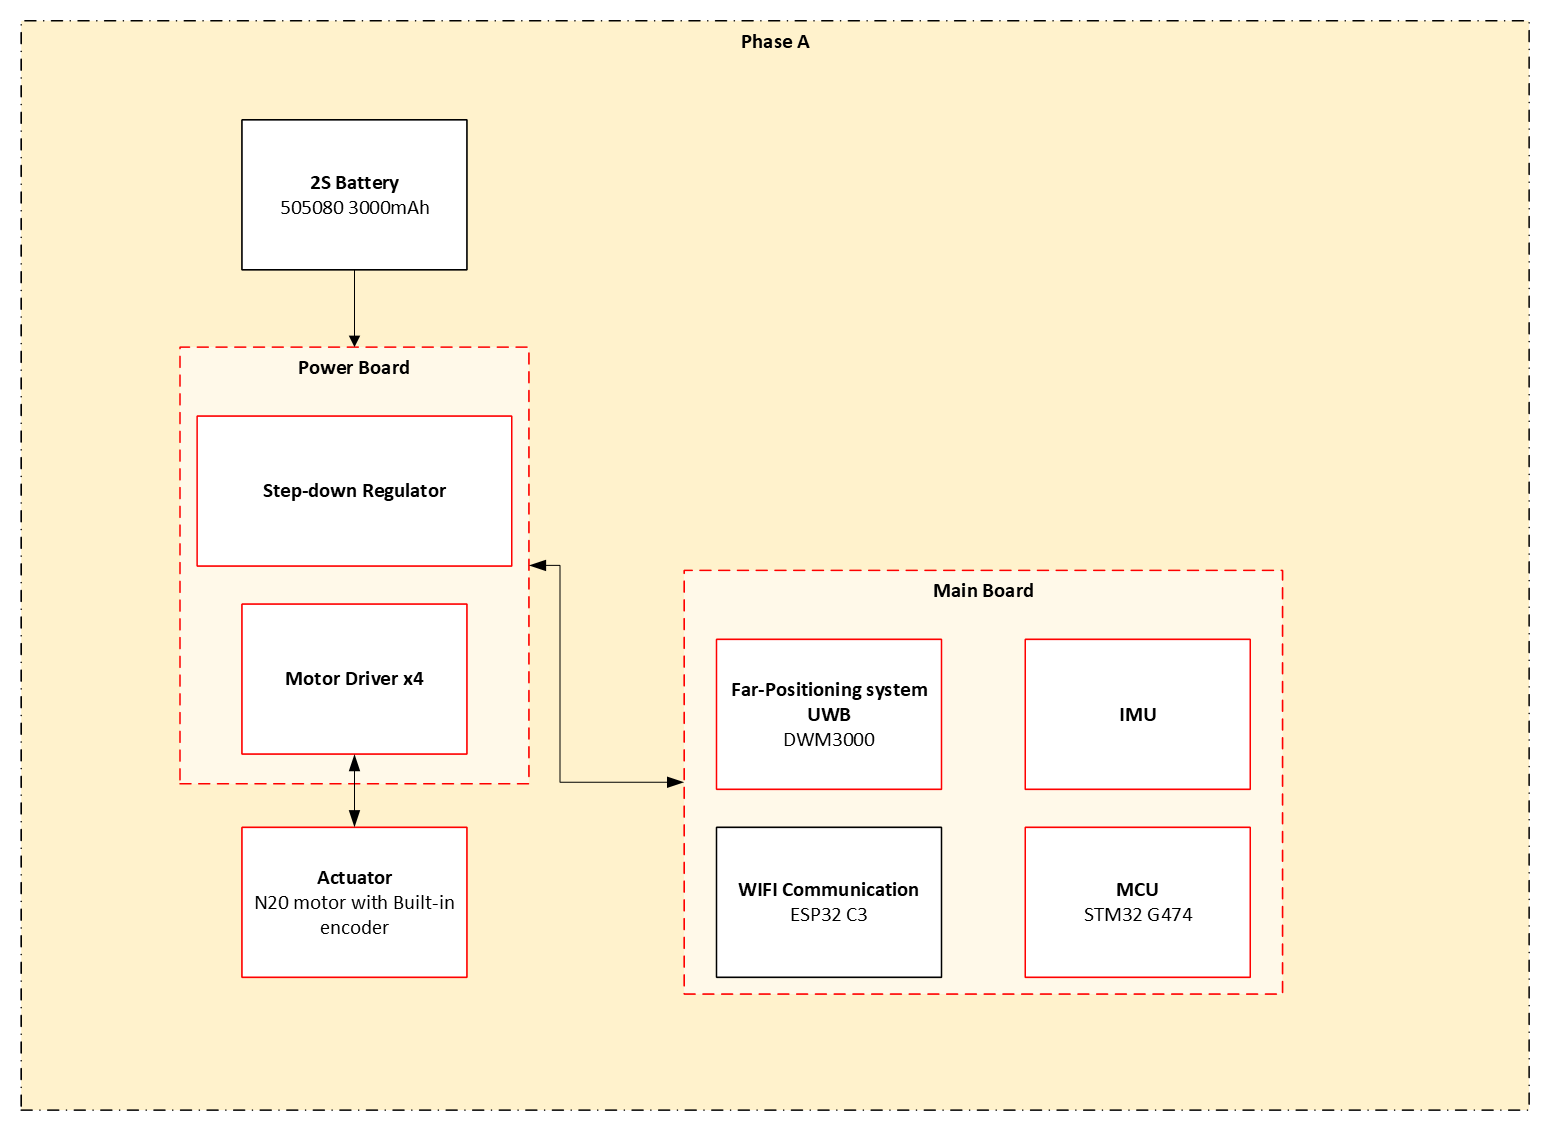
\includegraphics[width=0.78\textwidth]{image/Phase_A_Diagram.png}
		\caption{Phase A.}
		\label{fig:phase-a}
	\end{subfigure}
	\par\vspace{8pt}
	\begin{subfigure}[b]{\textwidth}
		\centering
		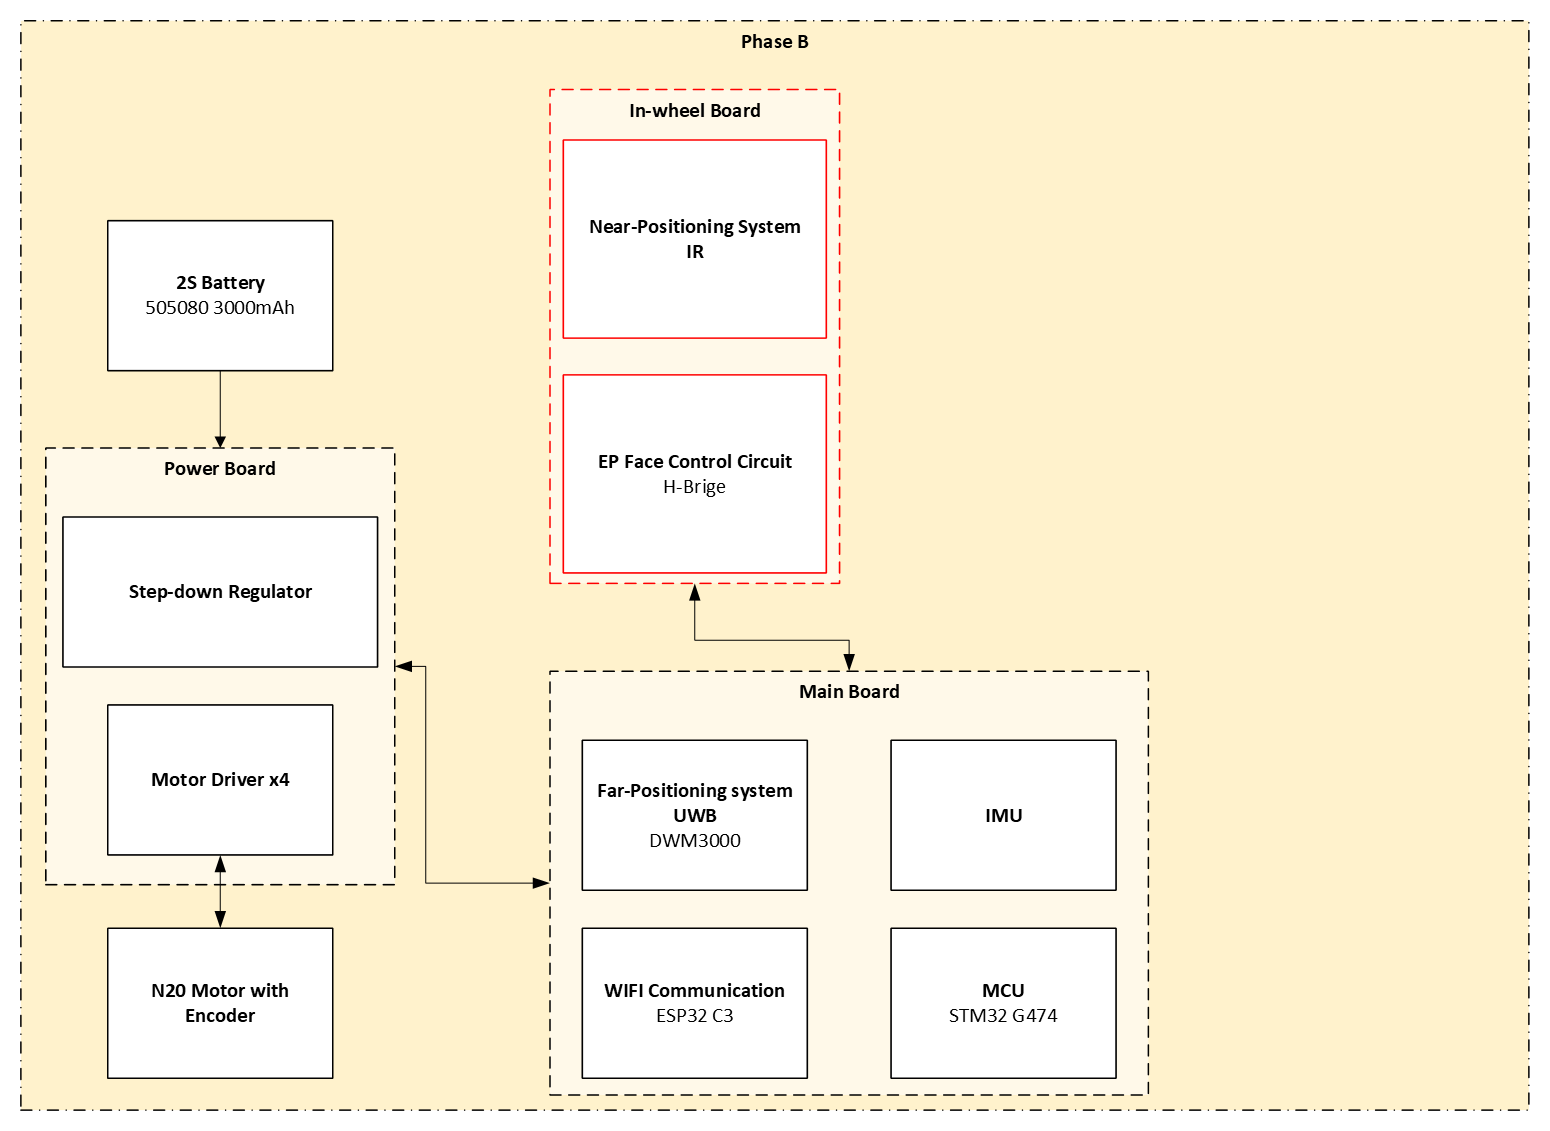
\includegraphics[width=0.78\textwidth]{image/Phase_B_Diagram.png}
		\caption{Phase B.}
		\label{fig:phase-b}
	\end{subfigure}
	\caption{Electronics block diagrams, Phases A--B.}
	\label{fig:phase-diagrams-ab}
\end{figure}

\begin{figure}[!htbp]
	\centering
	\begin{subfigure}[b]{\textwidth}
		\centering
		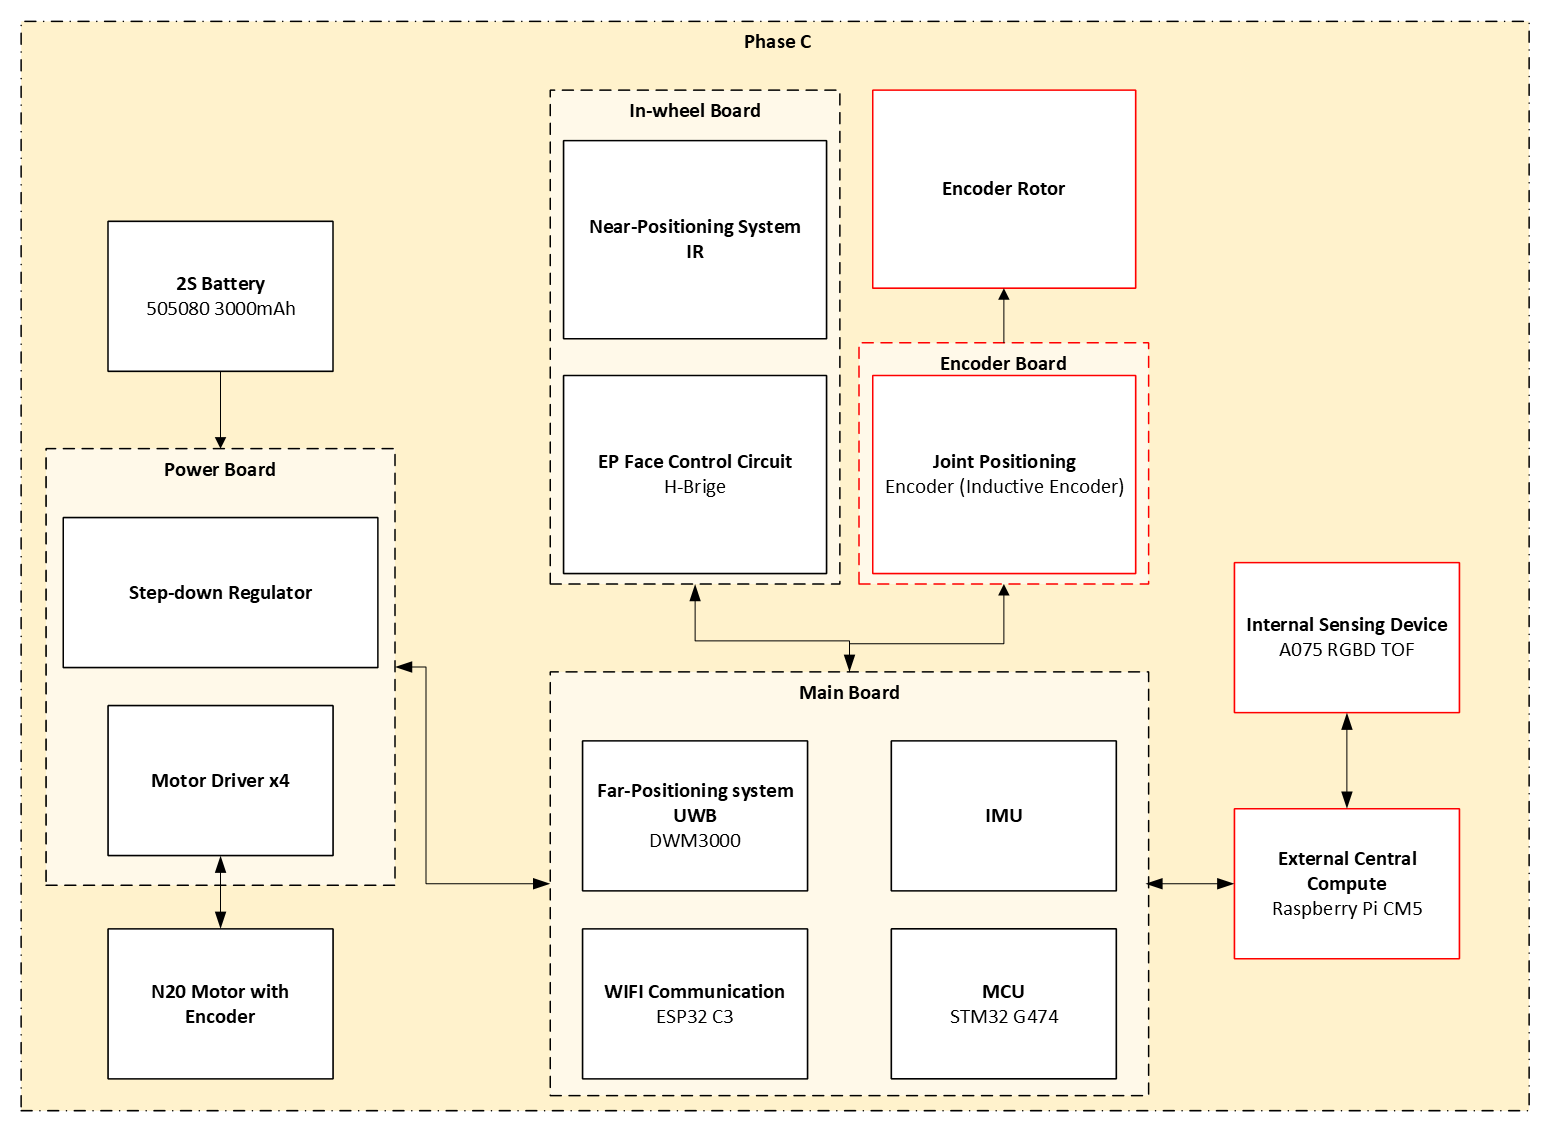
\includegraphics[width=0.78\textwidth]{image/Phase_C_Diagram.png}
		\caption{Phase C.}
		\label{fig:phase-c}
	\end{subfigure}
	\par\vspace{8pt}
	\begin{subfigure}[b]{\textwidth}
		\centering
		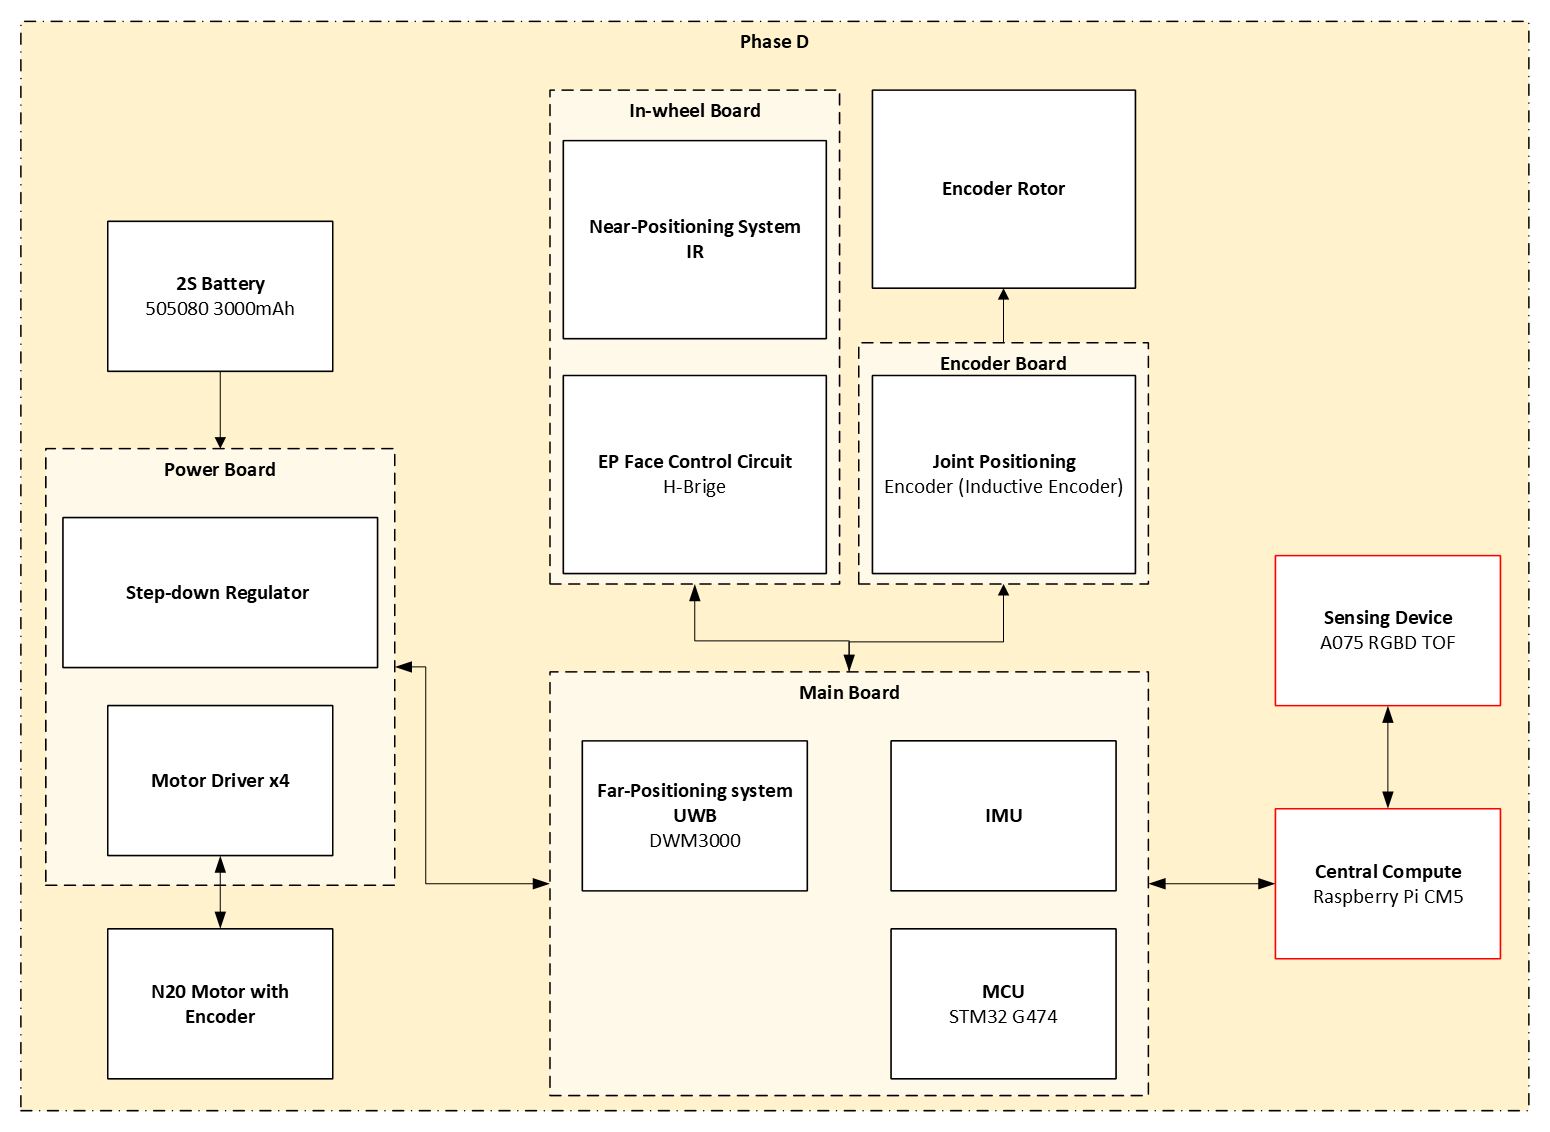
\includegraphics[width=0.78\textwidth]{image/Phase_D_Diagram.png}
		\caption{Phase D.}
		\label{fig:phase-d}
	\end{subfigure}
	\caption{Electronics block diagrams, Phases C--D.}
	\label{fig:phase-diagrams-cd}
\end{figure}

% ----------------------------------------------------------------
\subsection{Component Selection}

\begin{table}[H]
\centering\small
\caption{Key electronics components.}
\label{tab:components}
\begin{tabular}{@{}L{0.18\textwidth} L{0.15\textwidth} L{0.35\textwidth} L{0.22\textwidth}@{}}
\toprule
\textbf{Component} & \textbf{Phase} & \textbf{Key Specs} & \textbf{Interface / Supply} \\
\midrule
4$\times$ N20 gearmotor & A-1+ & 6\,V, 50\,rpm; 7\,PPR encoder & A/B quadrature; H-bridge \\
STM32G474 & A+ & Cortex-M4F @ 170\,MHz; 12-bit ADC; FDCAN & SPI/I2C/UART/CAN; 3.3\,V \\
ICM-42688-P & A+ & $\pm$2000\,dps / $\pm$16\,g; 32\,kHz ODR & SPI or I2C; 1.8\,V \\
DW3000 (UWB) & A+ & IEEE 802.15.4z; $\sim$10\,cm ranging & SPI; 3.3\,V \\
ESP32-C3 & A-1+ & Wi-Fi 4 + BLE 5; RISC-V @ 160\,MHz & UART/SPI; 3.3\,V \\
EP-Face + IR PCB & B & Custom; EP magnet + IR alignment & Slip ring; 3.3\,V \\
RPi CM5 & D & Cortex-A76 @ 2.4\,GHz; up to 16\,GB RAM & Custom carrier; 5\,V \\
Sipeed MaixSense A075V & C+ & ToF 320$\times$240 @ 30\,fps; RGB 800$\times$600 & USB 2.0; 5\,V \\
\bottomrule
\end{tabular}
\end{table}

% ----------------------------------------------------------------
\subsection{Electronics Packaging}

All components fit within the \SI{100}{mm} cube based on rough CAD placement (Figure~\ref{fig:elec-packaging}).

\begin{figure}[!htbp]
	\centering
	\begin{subfigure}[b]{0.45\textwidth}
		\centering
		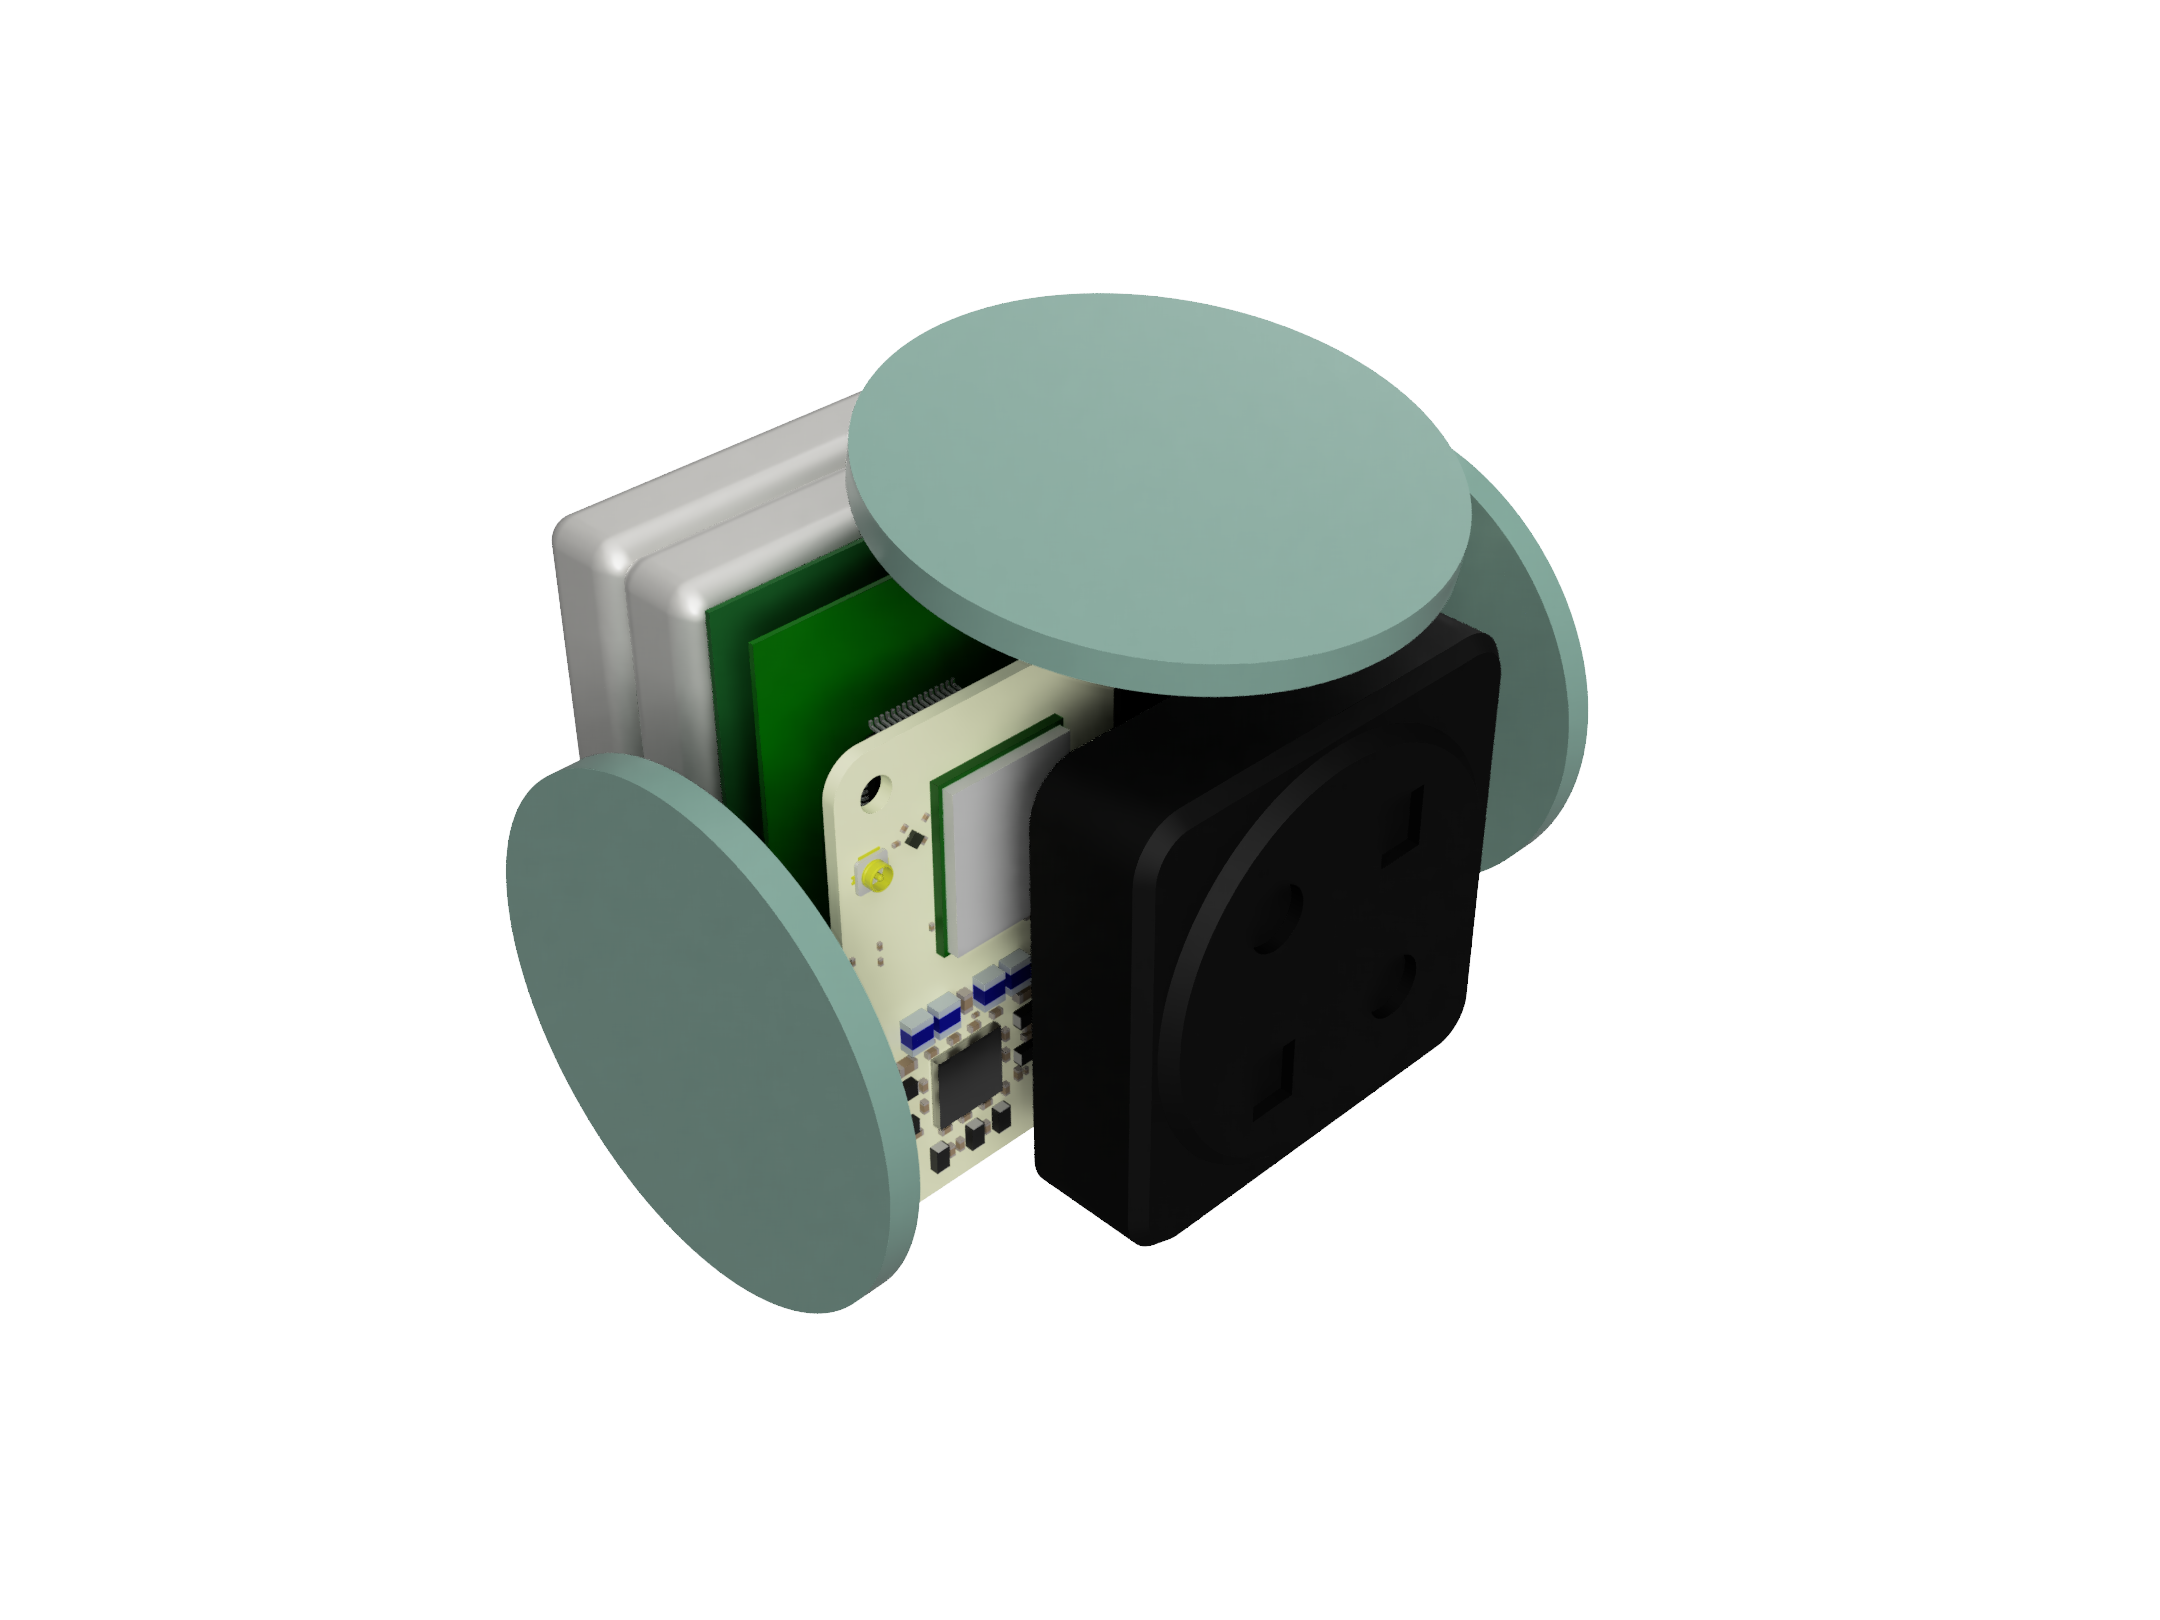
\includegraphics[width=\linewidth]{image/Elec_Assembly.png}
		\caption{Assembled.}
		\label{fig:elec-assembly}
	\end{subfigure}
	\hfill
	\begin{subfigure}[b]{0.45\textwidth}
		\centering
		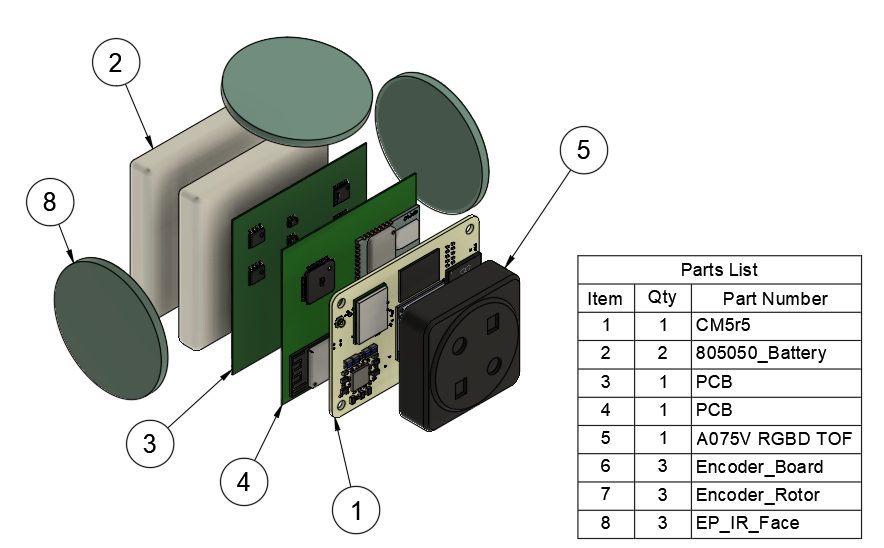
\includegraphics[width=\linewidth]{image/Elec_Exploded_View.png}
		\caption{Exploded.}
		\label{fig:elec-exploded}
	\end{subfigure}
	\caption{Electronics packaging.}
	\label{fig:elec-packaging}
\end{figure}

% ----------------------------------------------------------------
\subsection{Wheel Encoder}

Replacing the original continuous-rotation potentiometer ($\sim$5$^\circ$ resolution, contact wear) with a non-contact encoder. Three options considered:

\begin{table}[H]
\centering\small
\caption{Wheel encoder options.}
\label{tab:encoders}
\begin{tabular}{@{}L{0.20\textwidth} L{0.24\textwidth} L{0.24\textwidth} L{0.24\textwidth}@{}}
\toprule
& \textbf{On-axis magnetic} (AS5600) & \textbf{Off-axis tape} & \textbf{Custom inductive} \\
\midrule
Output & Absolute, 12--14 bit & Incremental + index & Absolute \\
EP interference & Sensitive & Sensitive & Immune \\
Design effort & Low & Medium & High \\
\bottomrule
\end{tabular}
\end{table}

The inductive option best handles the EP connector's nearby field but has the highest schedule risk. Decision deferred to Phase C.

% ----------------------------------------------------------------
\subsection{Power System}

\begin{figure}[!htbp]
  \centering
  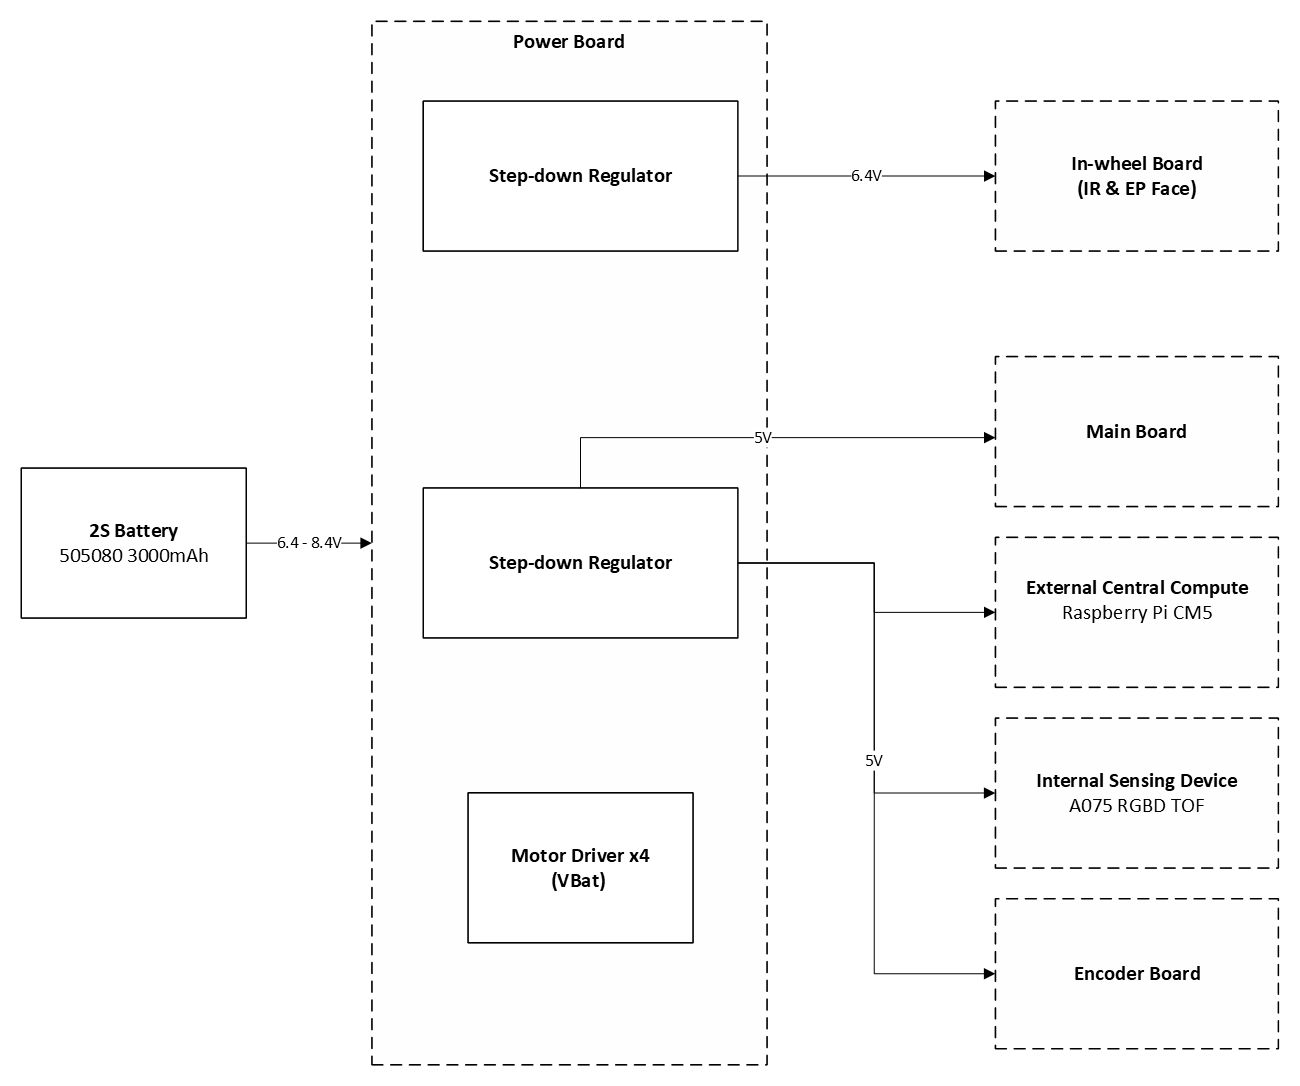
\includegraphics[width=0.6\textwidth]{image/Power_Diagram.png}
  \caption{Power distribution block diagram.}
  \label{fig:power-diagram}
\end{figure}

Power from a 2S LiPo (3000\,mAh, 22.2\,Wh) splits three ways:
\begin{itemize}
  \item \textbf{Motors:} 4$\times$ N20 via H-bridges, PWM capped at $\sim$70\,\% for 6\,V rating.
  \item \textbf{EP-Face:} Dedicated buck regulator isolates pulse transients from logic rail.
  \item \textbf{Logic/compute:} Buck to 5\,V (CM5, camera); LDO to 3.3\,V (MCU, sensors, radios).
\end{itemize}

\begin{table}[H]
\centering\small
\caption{Power budget summary.}
\label{tab:power-summary}
\begin{tabular}{@{}lcc@{}}
\toprule
\textbf{Configuration} & \textbf{Total from Pack} & \textbf{Est.\ Run Time} \\
\midrule
Phase A--B (no compute/camera) & $\sim$3.1\,W & $\sim$\textbf{5.8\,h} \\
Phase D (full system) & $\sim$11.5\,W & $\sim$\textbf{1.5\,h} \\
\bottomrule
\end{tabular}
\end{table}

\begin{table}[H]
\centering\small
\caption{Maximum load per rail.}
\label{tab:rail-max}
\begin{tabular}{@{}lcc@{}}
\toprule
\textbf{Rail} & \textbf{Max Current} & \textbf{Max Power} \\
\midrule
Motor drive (PWM to 6\,V) & 4.0\,A (6\,V eq.) & 24\,W \\
5\,V logic/compute & 4.0\,A & 20\,W \\
3.3\,V (from 5\,V LDO) & 0.45\,A & 1.5\,W \\
EP-Face + IR & TBD & TBD \\
\midrule
\textbf{Pack total (peak)} & $\sim$6.5\,A @ 7.4\,V & $\sim$47\,W \\
\bottomrule
\end{tabular}
\end{table}

\clearpage
% ================================================================
\section{Shaft Tolerance Analysis ($\varnothing$\SI{55}{mm} Bearing)}
\label{sec:shaft-tolerance}
% ================================================================

The plain bearing (OD = \SI{55}{mm}) acts as the shaft. All nylon-printed components have bores around it.

\begin{figure}[!htbp]
	\centering
	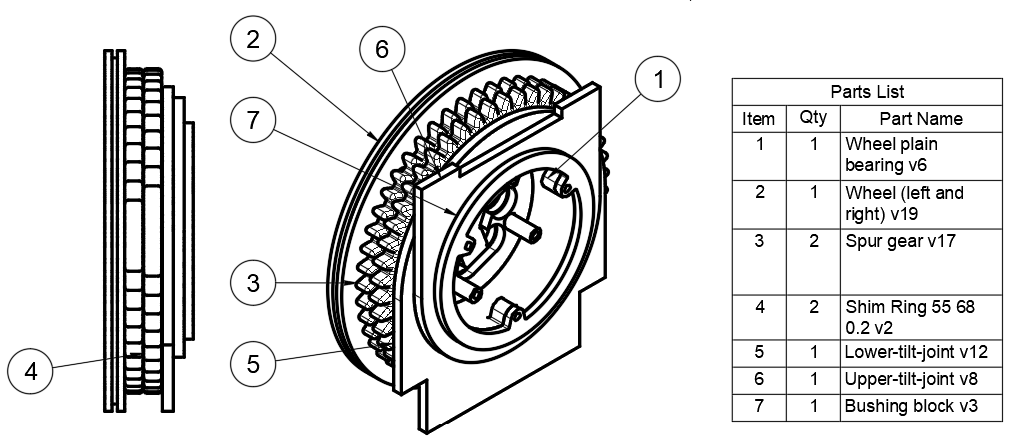
\includegraphics[width=0.6\textwidth]{image/shaft_component.png}
	\caption{Shaft and bearing component arrangement.}
	\label{fig:shaft-component}
\end{figure}

\begin{table}[H]
\centering
\caption{Joint classification and ISO fits for $\varnothing$\SI{55}{mm} bearing.}
\label{tab:shaft-joints}
\begin{tabular}{@{}cllll@{}}
\toprule
\textbf{Joint} & \textbf{Component} & \textbf{Motion} & \textbf{Fit} & \textbf{ISO Class} \\
\midrule
J1 & Wheel + 1\textsuperscript{st} Spur Gear & Dynamic & Clearance & F7/h6 \\
J2 & 2\textsuperscript{nd} Spur Gear (Pan/Tilt) & Dynamic & Clearance & F7/h6 \\
J3 & Upper Tilt Joint & Dynamic & Clearance & F7/h6 \\
J4 & Lower Tilt Joint & \textbf{Static} & \textbf{Interference} & P7/h6 \\
\bottomrule
\end{tabular}
\end{table}

\textbf{ISO\,286 limits} (bearing h6: $55.000$--$54.981$\,mm): Dynamic F7 bore $55.030$--$55.060$\,mm (clearance $+0.030$ to $+0.079$\,mm); Static P7 bore $54.938$--$54.968$\,mm (interference $+0.013$ to $+0.062$\,mm).

\textbf{FDM nylon compensation:} Printed holes shrink $\sim$0.10--0.30\,mm. Dynamic bores get $+0.20$\,mm compensation; static bores get $+0.10$\,mm (shrinkage helps create interference).

\begin{table}[H]
\centering
\caption{Recommended CAD bore sizes.}
\label{tab:shaft-quickref}
\renewcommand{\arraystretch}{1.3}
\begin{tabular}{@{}llcc@{}}
\toprule
\textbf{Part} & \textbf{Joint} & \textbf{CAD Bore (mm)} & \textbf{Expected Fit} \\
\midrule
Wheel / Spur Gears / Upper Tilt & J1--J3 Dynamic & $\varnothing 55.30$ & $\approx 0.10$--$0.20$ CL \\
Lower Tilt Joint & J4 \textbf{Static} & $\varnothing 54.90$ & $\approx 0.05$--$0.15$ IF \\
\bottomrule
\multicolumn{4}{@{}l}{\footnotesize CL = Clearance \quad IF = Interference \quad Bearing OD = $\varnothing 55.00$\,mm}
\end{tabular}
\end{table}

\textbf{Test plan:} Print nylon test rings at five bore sizes per fit type (dynamic: 55.10--55.50\,mm; static: 54.70--55.10\,mm). Cool $\geq$2\,h, measure with caliper at 3 angles. Pick smallest dynamic bore that spins freely; largest static bore that prevents rotation.

\clearpage
% ================================================================
\section{Software Testing Plan (Phase A)}
\label{sec:software-testing}

\subsection{Objectives}

Verify the integrated software pipeline: AprilTag detection and robot ID via external camera $\rightarrow$ real-time pose estimation $\rightarrow$ PID motor control $\rightarrow$ path planning and execution for MSRR configurations.

\subsection{Setup}

MSRR robot in a controlled indoor environment with an external camera, AprilTags for ID and pose reference, and a computing system running perception, localisation, planning, and control.

\subsection{Goal Configurations}

Snake, Car, DoubleDriver, L-shape.

\subsection{Evaluation Metrics}

\begin{itemize}
\item \textbf{Detection rate} --- \% frames with correct AprilTag ID.
\item \textbf{Position / orientation error} --- estimated vs.\ reference pose.
\item \textbf{Tracking error} --- desired vs.\ actual position and heading during path following.
\item \textbf{Control response} --- PID overshoot and steady-state error.
\item \textbf{Processing rate} --- perception + control update frequency.
\end{itemize}

\subsection{Acceptance Criteria}

Reliable tag detection, acceptable localisation and tracking error for real-time control, stable PID behaviour without excessive oscillation, and continuous operation without critical failures. Specific numerical thresholds to be defined based on system requirements.

\clearpage
% ================================================================
\section{Preparation for Phase B: EP Magnet}
\label{sec:phase-b-magnet}

The docking system uses an Electro-Permanent Magnet (EPM) connector based on SMORES-EP \cite{tosun2016}. Each EP unit pairs an AlNiCo~5 magnet (low coercivity, switchable) with an NdFeB magnet (high coercivity, fixed) between steel pole pieces, wound with a copper coil.

\begin{figure}[!htbp]
	\centering
	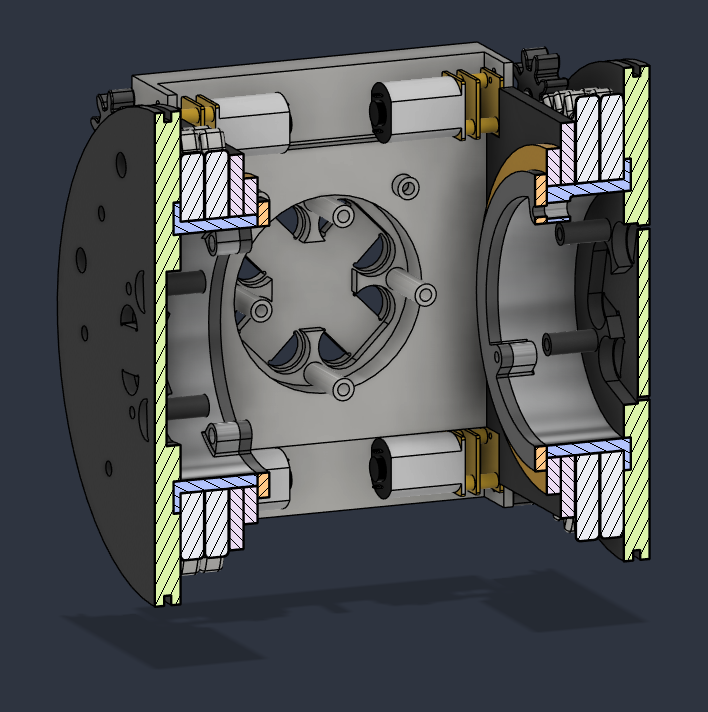
\includegraphics[width=0.6\textwidth]{image/inside_rectangular_magnet_housing.png}
	\caption{Interior view of the rectangular magnet housing.}
	\label{fig:cad-magnet-housing}
\end{figure}

\textbf{Operating principle:} A current pulse through the coil reverses AlNiCo~5 magnetisation while NdFeB stays fixed. Fields aligned $\rightarrow$ \textbf{ON} (attract); fields opposed $\rightarrow$ \textbf{OFF} (release). No power needed to hold either state.

\textbf{Materials:} AlNiCo~5 rod, NdFeB magnet, mild steel 1018/S20C pole pieces, 30~AWG enamelled copper wire (200 turns). Original dimensions (4.76\,mm dia.\ $\times$ 9.53\,mm, four magnets in 42\,mm ring) being adapted for the \SI{100}{mm} face. Final dimensions and driving circuit to be set in Phase~B testing.

% 

\renewcommand{\refname}{Additional References}
\begin{thebibliography}{9}

\bibitem{tosun2016}
Tosun, T., Davey, J., Liu, C., \& Yim, M. (2016). Design and characterization
of the EP-Face connector. In \textit{IEEE/RSJ International Conference on
Intelligent Robots and Systems (IROS)} (pp.\ 45--51).

\end{thebibliography}

\end{document}